\documentclass{standalone}
\usepackage{tikz}
\usetikzlibrary{patterns, positioning}

\begin{document}
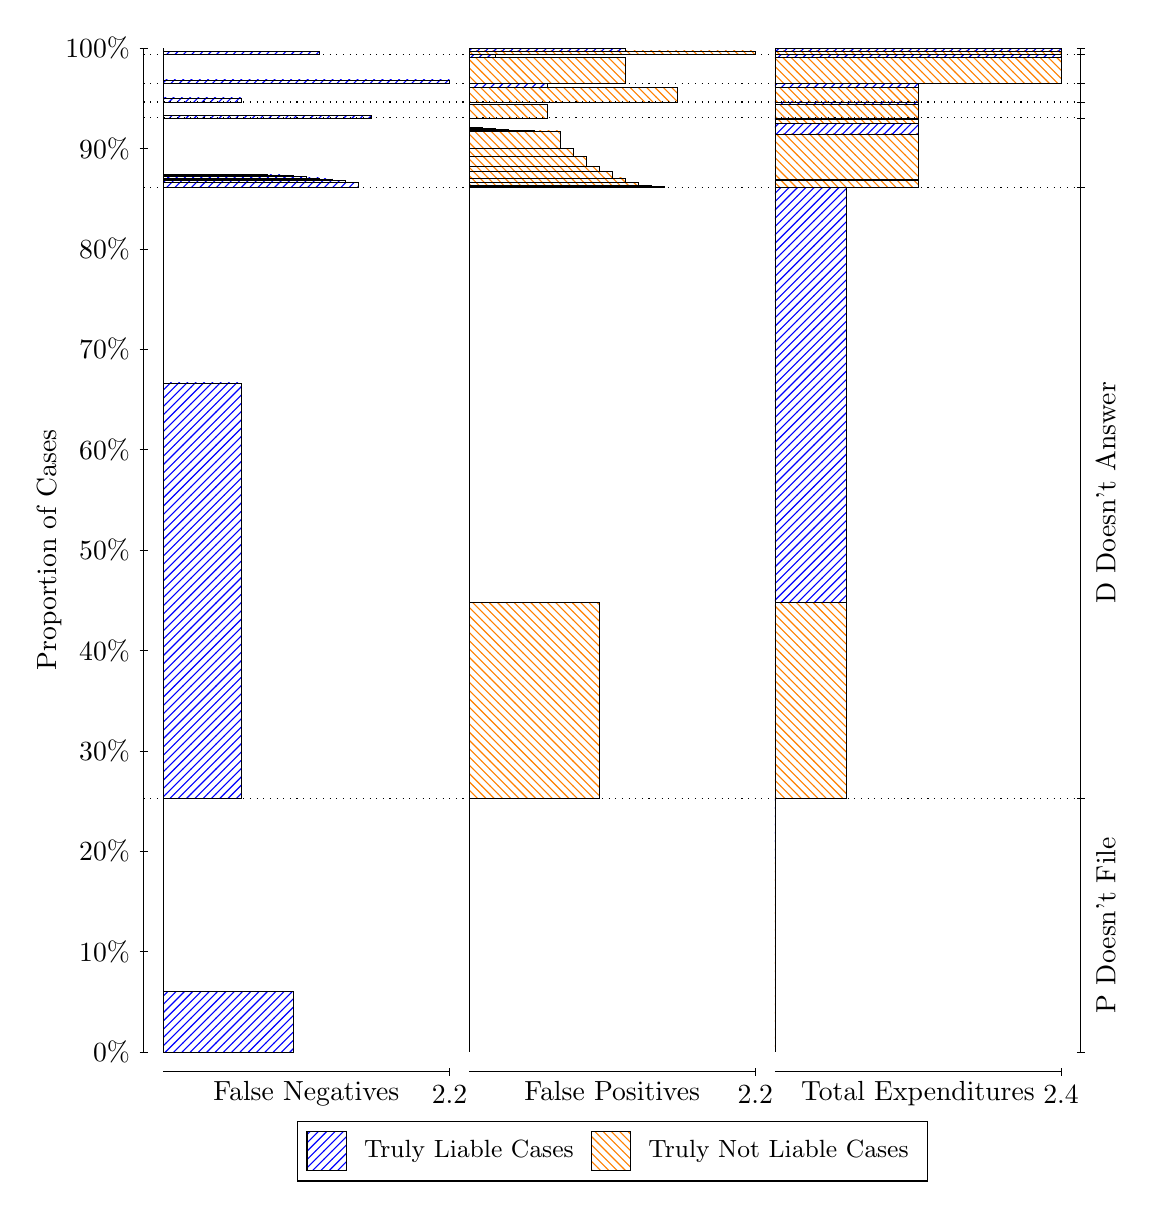
\begin{tikzpicture}
\draw[black, very thin] (1.5,1.75) -- (1.5,14.5);
\node[rotate=90, anchor=center] at (0.3, 8.125) {Proportion of Cases};
\draw[black, very thin] (1.45,1.75) -- (1.55,1.75);
\node[anchor=east] at (1.45, 1.75) {0\%};
\draw[black, very thin] (1.45,3.025) -- (1.55,3.025);
\node[anchor=east] at (1.45, 3.025) {10\%};
\draw[black, very thin] (1.45,4.3) -- (1.55,4.3);
\node[anchor=east] at (1.45, 4.3) {20\%};
\draw[black, very thin] (1.45,5.575) -- (1.55,5.575);
\node[anchor=east] at (1.45, 5.575) {30\%};
\draw[black, very thin] (1.45,6.85) -- (1.55,6.85);
\node[anchor=east] at (1.45, 6.85) {40\%};
\draw[black, very thin] (1.45,8.125) -- (1.55,8.125);
\node[anchor=east] at (1.45, 8.125) {50\%};
\draw[black, very thin] (1.45,9.4) -- (1.55,9.4);
\node[anchor=east] at (1.45, 9.4) {60\%};
\draw[black, very thin] (1.45,10.675) -- (1.55,10.675);
\node[anchor=east] at (1.45, 10.675) {70\%};
\draw[black, very thin] (1.45,11.95) -- (1.55,11.95);
\node[anchor=east] at (1.45, 11.95) {80\%};
\draw[black, very thin] (1.45,13.225) -- (1.55,13.225);
\node[anchor=east] at (1.45, 13.225) {90\%};
\draw[black, very thin] (1.45,14.5) -- (1.55,14.5);
\node[anchor=east] at (1.45, 14.5) {100\%};

\draw[black, very thin] (13.4,1.75) -- (13.4,14.5);
\draw[black, very thin] (13.35,1.75) -- (13.45,1.75);
\node[anchor=west] at (13.35, 1.75) {};
\draw[black, very thin] (13.35,4.9709) -- (13.45,4.9709);
\node[anchor=west] at (13.35, 4.9709) {};
\draw[black, very thin] (13.35,12.732) -- (13.45,12.732);
\node[anchor=west] at (13.35, 12.732) {};
\draw[black, very thin] (13.35,13.614) -- (13.45,13.614);
\node[anchor=west] at (13.35, 13.614) {};
\draw[black, very thin] (13.35,13.815) -- (13.45,13.815);
\node[anchor=west] at (13.35, 13.815) {};
\draw[black, very thin] (13.35,14.051) -- (13.45,14.051);
\node[anchor=west] at (13.35, 14.051) {};
\draw[black, very thin] (13.35,14.422) -- (13.45,14.422);
\node[anchor=west] at (13.35, 14.422) {};
\draw[black, very thin] (13.35,14.5) -- (13.45,14.5);
\node[anchor=west] at (13.35, 14.5) {};

\draw[black, very thin, pattern color=blue, pattern=north east lines] (1.75,1.75) rectangle (3.4015,2.5226);
\draw[black, very thin, pattern color=orange, pattern=north west lines] (1.75,2.5226) rectangle (1.75,4.9709);
\draw[black, very thin, pattern color=blue, pattern=north east lines] (1.75,4.9709) rectangle (2.7409,10.248);
\draw[black, very thin, pattern color=orange, pattern=north west lines] (1.75,10.248) rectangle (1.75,12.732);
\draw[black, very thin, pattern color=blue, pattern=north east lines] (1.75,12.732) rectangle (4.2273,12.795);
\draw[black, very thin, pattern color=blue, pattern=north east lines] (1.75,12.795) rectangle (4.0621,12.816);
\draw[black, very thin, pattern color=blue, pattern=north east lines] (1.75,12.816) rectangle (3.897,12.838);
\draw[black, very thin, pattern color=blue, pattern=north east lines] (1.75,12.838) rectangle (3.7318,12.852);
\draw[black, very thin, pattern color=blue, pattern=north east lines] (1.75,12.852) rectangle (3.5667,12.871);
\draw[black, very thin, pattern color=blue, pattern=north east lines] (1.75,12.871) rectangle (3.4015,12.88);
\draw[black, very thin, pattern color=blue, pattern=north east lines] (1.75,12.88) rectangle (3.2364,12.89);
\draw[black, very thin, pattern color=blue, pattern=north east lines] (1.75,12.89) rectangle (3.0712,12.896);
\draw[black, very thin, pattern color=blue, pattern=north east lines] (1.75,12.896) rectangle (2.9061,12.898);
\draw[black, very thin, pattern color=orange, pattern=north west lines] (1.75,12.898) rectangle (1.75,13.614);
\draw[black, very thin, pattern color=blue, pattern=north east lines] (1.75,13.614) rectangle (4.3924,13.643);
\draw[black, very thin, pattern color=orange, pattern=north west lines] (1.75,13.643) rectangle (1.75,13.815);
\draw[black, very thin, pattern color=blue, pattern=north east lines] (1.75,13.815) rectangle (2.7409,13.867);
\draw[black, very thin, pattern color=orange, pattern=north west lines] (1.75,13.867) rectangle (1.75,14.051);
\draw[black, very thin, pattern color=blue, pattern=north east lines] (1.75,14.051) rectangle (5.3833,14.096);
\draw[black, very thin, pattern color=orange, pattern=north west lines] (1.75,14.096) rectangle (1.75,14.422);
\draw[black, very thin, pattern color=blue, pattern=north east lines] (1.75,14.422) rectangle (3.7318,14.457);
\draw[black, very thin, pattern color=orange, pattern=north west lines] (1.75,14.457) rectangle (1.75,14.5);
\draw[black, very thin, pattern color=orange, pattern=north west lines] (5.6333,1.75) rectangle (5.6333,4.1983);
\draw[black, very thin, pattern color=blue, pattern=north east lines] (5.6333,4.1983) rectangle (5.6333,4.9709);
\draw[black, very thin, pattern color=orange, pattern=north west lines] (5.6333,4.9709) rectangle (7.2848,7.455);
\draw[black, very thin, pattern color=blue, pattern=north east lines] (5.6333,7.455) rectangle (5.6333,12.732);
\draw[black, very thin, pattern color=orange, pattern=north west lines] (5.6333,12.732) rectangle (8.1106,12.742);
\draw[black, very thin, pattern color=orange, pattern=north west lines] (5.6333,12.742) rectangle (7.9455,12.759);
\draw[black, very thin, pattern color=orange, pattern=north west lines] (5.6333,12.759) rectangle (7.7803,12.798);
\draw[black, very thin, pattern color=orange, pattern=north west lines] (5.6333,12.798) rectangle (7.6152,12.85);
\draw[black, very thin, pattern color=orange, pattern=north west lines] (5.6333,12.85) rectangle (7.45,12.935);
\draw[black, very thin, pattern color=orange, pattern=north west lines] (5.6333,12.935) rectangle (7.2848,12.998);
\draw[black, very thin, pattern color=orange, pattern=north west lines] (5.6333,12.998) rectangle (7.1197,13.127);
\draw[black, very thin, pattern color=orange, pattern=north west lines] (5.6333,13.127) rectangle (6.9545,13.227);
\draw[black, very thin, pattern color=orange, pattern=north west lines] (5.6333,13.227) rectangle (6.7894,13.448);
\draw[black, very thin, pattern color=blue, pattern=north east lines] (5.6333,13.448) rectangle (6.4591,13.45);
\draw[black, very thin, pattern color=blue, pattern=north east lines] (5.6333,13.45) rectangle (6.2939,13.456);
\draw[black, very thin, pattern color=blue, pattern=north east lines] (5.6333,13.456) rectangle (6.1288,13.466);
\draw[black, very thin, pattern color=blue, pattern=north east lines] (5.6333,13.466) rectangle (5.9636,13.475);
\draw[black, very thin, pattern color=blue, pattern=north east lines] (5.6333,13.475) rectangle (5.7985,13.494);
\draw[black, very thin, pattern color=blue, pattern=north east lines] (5.6333,13.494) rectangle (5.6333,13.614);
\draw[black, very thin, pattern color=orange, pattern=north west lines] (5.6333,13.614) rectangle (6.6242,13.787);
\draw[black, very thin, pattern color=blue, pattern=north east lines] (5.6333,13.787) rectangle (5.6333,13.815);
\draw[black, very thin, pattern color=orange, pattern=north west lines] (5.6333,13.815) rectangle (8.2758,14);
\draw[black, very thin, pattern color=blue, pattern=north east lines] (5.6333,14) rectangle (6.6242,14.051);
\draw[black, very thin, pattern color=orange, pattern=north west lines] (5.6333,14.051) rectangle (7.6152,14.378);
\draw[black, very thin, pattern color=blue, pattern=north east lines] (5.6333,14.378) rectangle (5.9636,14.422);
\draw[black, very thin, pattern color=orange, pattern=north west lines] (5.6333,14.422) rectangle (9.2667,14.465);
\draw[black, very thin, pattern color=blue, pattern=north east lines] (5.6333,14.465) rectangle (7.6152,14.5);
\draw[black, very thin, pattern color=orange, pattern=north west lines] (9.5167,1.75) rectangle (9.5167,4.1983);
\draw[black, very thin, pattern color=blue, pattern=north east lines] (9.5167,4.1983) rectangle (9.5167,4.9709);
\draw[black, very thin, pattern color=orange, pattern=north west lines] (9.5167,4.9709) rectangle (10.425,7.455);
\draw[black, very thin, pattern color=blue, pattern=north east lines] (9.5167,7.455) rectangle (10.425,12.732);
\draw[black, very thin, pattern color=orange, pattern=north west lines] (9.5167,12.732) rectangle (11.333,12.816);
\draw[black, very thin, pattern color=blue, pattern=north east lines] (9.5167,12.816) rectangle (11.333,12.835);
\draw[black, very thin, pattern color=orange, pattern=north west lines] (9.5167,12.835) rectangle (11.333,13.411);
\draw[black, very thin, pattern color=blue, pattern=north east lines] (9.5167,13.411) rectangle (11.333,13.543);
\draw[black, very thin, pattern color=orange, pattern=north west lines] (9.5167,13.543) rectangle (11.333,13.598);
\draw[black, very thin, pattern color=blue, pattern=north east lines] (9.5167,13.598) rectangle (11.333,13.614);
\draw[black, very thin, pattern color=orange, pattern=north west lines] (9.5167,13.614) rectangle (11.333,13.787);
\draw[black, very thin, pattern color=blue, pattern=north east lines] (9.5167,13.787) rectangle (11.333,13.815);
\draw[black, very thin, pattern color=orange, pattern=north west lines] (9.5167,13.815) rectangle (11.333,14);
\draw[black, very thin, pattern color=blue, pattern=north east lines] (9.5167,14) rectangle (11.333,14.051);
\draw[black, very thin, pattern color=orange, pattern=north west lines] (9.5167,14.051) rectangle (13.15,14.378);
\draw[black, very thin, pattern color=blue, pattern=north east lines] (9.5167,14.378) rectangle (13.15,14.422);
\draw[black, very thin, pattern color=orange, pattern=north west lines] (9.5167,14.422) rectangle (13.15,14.465);
\draw[black, very thin, pattern color=blue, pattern=north east lines] (9.5167,14.465) rectangle (13.15,14.5);
\draw[black, dotted] (1.5,4.9709) -- (13.4,4.9709);
\draw[black, dotted] (1.5,12.732) -- (13.4,12.732);
\draw[black, dotted] (1.5,13.614) -- (13.4,13.614);
\draw[black, dotted] (1.5,13.815) -- (13.4,13.815);
\draw[black, dotted] (1.5,14.051) -- (13.4,14.051);
\draw[black, dotted] (1.5,14.422) -- (13.4,14.422);
\draw[black, very thin] (1.75,1.5) -- (5.3833,1.5);
\node[anchor=north] at (3.5667, 1.5) {False Negatives};
\draw[black, very thin] (5.3833,1.45) -- (5.3833,1.55);
\node[anchor=north] at (5.3833, 1.45) {2.2};

\draw[black, very thin] (5.6333,1.5) -- (9.2667,1.5);
\node[anchor=north] at (7.45, 1.5) {False Positives};
\draw[black, very thin] (9.2667,1.45) -- (9.2667,1.55);
\node[anchor=north] at (9.2667, 1.45) {2.2};

\draw[black, very thin] (9.5167,1.5) -- (13.15,1.5);
\node[anchor=north] at (11.333, 1.5) {Total Expenditures};
\draw[black, very thin] (13.15,1.45) -- (13.15,1.55);
\node[anchor=north] at (13.15, 1.45) {2.4};

\node[black, centered, rotate=90] at (13.72, 3.3605) {P Doesn't File};
\node[black, centered, rotate=90] at (13.72, 8.8513) {D Doesn't Answer};






\draw (7.449999999999999,1.5) node[draw=none] (baseCoordinate) {};
\begin{scope}[align=center]
        \matrix[scale=0.5, draw=black, below=0.5cm of baseCoordinate, nodes={draw}, column sep=0.1cm]{
            \node[rectangle, draw, minimum width=0.5cm, minimum height=0.5cm, pattern=north east lines, pattern color=blue] {}; &
            \node[draw=none, font=\small] (B) {Truly Liable Cases}; &
            \node[rectangle, draw, minimum width=0.5cm, minimum height=0.5cm, pattern=north west lines, pattern color=orange] {}; &
            \node[draw=none, font=\small] (B) {Truly Not Liable Cases}; \\
            };
\end{scope}

\end{tikzpicture}
\end{document}